\documentclass[conference]{IEEEtran}
\IEEEoverridecommandlockouts
% The preceding line is only needed to identify funding in the first footnote. If that is unneeded, please comment it out.
\usepackage{amsmath,amssymb,amsfonts}
\usepackage{algorithmic}
\usepackage{graphicx}
\usepackage{textcomp}
\usepackage{xcolor}
\usepackage{amsmath}
\usepackage{tabularx}
\usepackage[style=ieee,sortcites=true,maxbibnames=100]{biblatex}
\usepackage{float}
\def\BibTeX{{\rm B\kern-.05em{\sc i\kern-.025em b}\kern-.08em
    T\kern-.1667em\lower.7ex\hbox{E}\kern-.125emX}}


\addbibresource{../bibtex.bib}

\begin{document}

\title{Improving the energy efficiency of battery powered WiFi sensors.\\
{\footnotesize \textsuperscript{*}Using the ESP8266-01 MCU as an example.}
% \thanks{Identify applicable funding agency here. If none, delete this.}
}

\author{\IEEEauthorblockN{Roland Rauter}
\IEEEauthorblockA{\textit{Management Center Innsbruck} \\
\textit{DiBSE}\\
Innsbruck, Austria \\
roland97@gmx.at}
\and
\IEEEauthorblockN{Arthur Waldner}
\IEEEauthorblockA{\textit{Management Center Innsbruck} \\
\textit{DiBSE}\\
Innsbruck, Austria \\
arthur.waldner@outlook.com}
\and
\IEEEauthorblockN{Thomas Widmann}
\IEEEauthorblockA{\textit{Management Center Innsbruck} \\
\textit{DiBSE}\\
Innsbruck, Austria \\
thomas.widmann@icloud.com}
}

\maketitle

\begin{abstract}
As IoT devices gain on popularity in sectors such as healthcare and smart home environments and as a lot of these IoT devices are battery powered and difficult to reach and maintain, it's crucial for them to have a long battery life.
Per definition, an IoT device has to connect with other devices or the internet. 
There are many communication protocols available to perform this task, but in our case we use WiFi because this technology is present in almost every home and most smart home applications use this technology.
In order to increase the battery life of such IoT devices, there are a lot of possible options available.
Three of these possible options are evaluated and described. Their impact on the energy efficiency is shown by conducting experiments.
Our results showed that using the deep sleep mode of the controller, improves the power consumption by a factor of $\approx 290$ compared to the modem sleep mode.


\end{abstract}

\begin{IEEEkeywords}
ESP8266, WiFi, MCU, IoT, Low power sensor
\end{IEEEkeywords}

\section{Introduction}

IoT is an evergrowing technology and it is estimated that in 2025, 75.4 billion IoT devices will be installed around the globe \cite{lucero2016iot}. These devices can be used in a wide range of life applications such as healthcare, transportaion, logistics and even in personal smart home environments.\\  
In order to declare a microcontroller or in general, a programmable device, an IoT device, it needs to communicate in some sort to the internet or to other devices. There are numerous communication protocols available to do that job. Some examples are ZigBee, BLE, Z-Wave, NFC and WiFi \cite{8079928}. 
When choosing a suitable connection protocol for a battery powered IoT device, the already available communication protocols and their energy consumption should be considered.\\
In our research paper, we investigate the different methods to extend the battery life of IoT devices with WiFi communication, because WiFi is the most common communication protocol that's available in nearly all households and we want this paper to be in context of smart home applications.\\
A part of a smart home environment can be described as Wireless sensor network. A Wireless sensor network consists of battery powered stand-alone devices with few sensors on them, with limitied processing power and an interface that allows them to communicate with each other \cite{wsn}. 
An example for WSN in smart home would be a battery powered ESP8266 with a temperature sensor on it, that sends data via MQTT to other devices.
MQTT is a light weight Message Queuing Telemetry Transport (MQTT) protocol which can be used perfectly with the ESP8266 because of it's light weight and small energy consumption \cite{kodali_mqtt_2016}.\\
In this paper, we evaluate three categories of methods to increase the battery life of the ESP8266 connected via WiFi and their impact on the energy efficiency.
These three questions are asked and evaluated: Do the different sleep modes of the ESP8266 improve the energy efficiency?, does the usage of a static IP instead of DHCP improve the energy efficiency?, is there a difference of using UDP instead of TCP?


\section{Theoretical background}

\subsection{Sleep modes}
Sleep modes are a very common way to improve the energy efficiency of micro controllers.
The basic idea is to reduce the power consumption by disabling unused modules in the chip and only power them up when they are needed.
In the case of the ESP8266, the vendor provides three different sleep modes. 
Table \ref{tab_sleep_modes} summarises the capabilities and typical current consumptions of the available sleep modes.
\cite{mesquita_assessing_2018}

\begin{table}[htbp]
\caption{ESP8266 sleep modes}
\begin{center}
\begin{tabular}{|c|c|c|c|}
\hline
\textbf{Module}&\textbf{Modem sleep}&\textbf{Light sleep}&\textbf{Deep sleep}\\
\hline
\textbf{WiFi} & OFF & OFF & OFF\\
\textbf{AP association} & Connected & Connected & Disconnected\\
\textbf{System clock} & ON & OFF & OFF\\
\textbf{RTC} & ON & ON & ON\\
\textbf{CPU} & ON & Pending & OFF\\
\hline
\textbf{Substrate current} & $15mA$ & $0.4mA$ & $20\mu A$\\
\hline
\end{tabular}
\label{tab_sleep_modes}
\end{center}
\end{table}

\subsubsection{Modem sleep} \label{sec:modem_sleep}
Modem sleep is the default sleep mode of the ESP8266 and is recommended for applications that require a real time CPU control. \cite{mesquita_assessing_2018}
By enabling the modem sleep, the ESP8266 will turn off the WiFi modem between the DTIM beacons. 
This improves the power consumption of the system and has the advantage that the system stays connected to the AP.\\
A typical use case is a WiFi controlled light bulb that provides real time light control.\cite{espressif_inc_esp8266_2016}

\subsubsection{Light sleep} \label{sec:light_sleep}
The light sleep mode is similar to the modem sleep mode with the additional improvement that the internal clock is powered off and the CPU is suspended when there are no tasks to execute.\\
According to the datasheet \cite{espressif_inc_esp8266_2016}, it takes less than $3ms$ to switch back into modem sleep mode.\\
This mode can be used when the application needs to stay connected to the access point 
and needs to responde to incoming data. The CPU is powered off when no data receives.

\subsubsection{Deep sleep} \label{sec:deep_sleep}
For ultra low power applications, the ESP8266 provides a deep sleep mode.
In this mode are all modules disabled except the real time clock (RTC) which can be used to wake up the controller periodically.
When the controller is in the deep sleep mode, it can only be woken up by applying a pulse to the RST pin.
This pulse can either be generated by an external device like a motion sensor or by the built in RTC module.\\
Another usefull feature is the RTC memory. This kind of memory makes it possible to store data over deep sleep cycles.
It losses the stored data only when the controller is disconnected from the power supply.
A possible use case is, to collect multiple measurement samples over time and send them out in a single package.\\
Deep sleep can be used for ultra low power applications that can be idle most of the time. 
However, there is the limitation that the system is not reachable from the outside at all times. \cite{espressif_inc_esp8266_2016}

\subsection{DHCP}
In order to connect the ESP8266 and in general every device with a Wi-Fi module to the Internet, it needs to have an IP-Address, so it can be identified by the router. 
There exist two possibilities to gain an IP-Address.\\ The first one is, to give the device a static IP-Address. As the name suggests, the IP-Address of the device will never change and it will be static. On the other hand, the IP-Address can be given dynamically.
The protocol, that gives dynamically IP-Addresses to the Wi-Fi clients is called DHCP (Dynamic Host Configuration Protocol).
It works as followed: When a device wants to connect to a network, a request to use an address for a time period to the DHCP server is sent. This time period is called "lease" \cite{droms1997rfc2131}. Then the DHCP server responds with the defined network configuration and an IP address.\\
The lease-time is defined by the DHCP server. When the time period is running out, the client has to send another request to the DHCP server. It's common that this happens after the half of the lease time.
Choosing the right lease-time depends on the given conditions. A huge factor is the size of the network and the grade of mobility of the connected devices. When there is a high number of mobile devices connected to the network and they don't stay very long in it. It's recommended that a shorter lease time is chosen, to prevent wasting valuable IP addresses in a sometimes small address pool \cite{khadilkar2007usage}.
But using a shorter lease-time leads to a bigger network overhead \cite{li_how_2018}. In further sequence, shorter lease times lead to more energy consumption of IoT devices, because the proccess of getting a new valid IP address takes energy.\\
It is proven that using a static IP address rather than using DHCP for IP address allocation is less energy consuming on IoT devices. Longer lease times can also improve the energy efficiency \cite{department_of_computer_engineering_mehmet_akif_ersoy_university_faculty_of_engineering_and_architecture_burdur_turkey_power_2020}. This understanding helps us to improve the energy efficiency on the ESP8266.





\subsection{UDP and TCP}
\label{udptcp:sci}
\subsubsection{TCP}
\label{tcp:sci}
Transmission Control Protocol is a connection-oriented network protocol
for sending data over a network.
This means that TCP waits until a connection is established and
then starts transmitting data\cite{postel1981transmission}.
TCP guaratees that data is transmitted to recipiend
in the correct order and without corrupt segments.
As a downside, this creates an enormous overhead compared
to other network protocols\cite{singh2014survey}\newline.
\subsubsection{UDP}
\label{udp:sci}
User Datagram Protocol is a connectionless network protocol
\cite{postel1980user}.
This protocol has no error handling or recovery options for
 the transmission and sends the data continuously.
It is not necessary for the sender that the client 
receives the data.
Compared to TCP, it allows less overhead when transferring data
\cite{singh2014survey}.

\section{Scientific approach}

To answer the questions, we conducted an experiment which is divided into three individual parts.
The independent variables are the three different sleep modes, how the WiFi connection is established (DHCP or static IP) and what transmission protocol is used to send the data (UDP or TCP).
We used DHCP with a random MAC address every time a connection is established, except when analyzing the behavior of using a static IP address.\\
The dependent variables are the current consumption in $mA$ and the energy consumption in $As$. Both of them are ratio scaled.
We used the ESP8266-01 microcontroller as main device and an FTDI (USB to serial) adapter to program it. 
For programming, we used the Arduino IDE in version 1.8.16.\\
When conducting, the impacts of different sleep modes, we used the setup described in Fig. \ref{fig:experiment_deep_sleep} and Fig. \ref{fig:experiment_modem_light_sleep}.\\
When conducting, the differences of using a static IP instead of DHCP, we used the setup described in Fig. \ref{fig:experiment_static_ip} and Fig. \ref{fig:experiment_deep_sleep}.\\
When conducting, if there's an impact on energy consumption when using UDP instead of TCP, we used the setup shown in Fig. \ref{fig:tcp_uml} and Fig. \ref{fig:udp_uml}.\\
During the experiment, the WiFi network operates like a normal network in a private household with several devices connected, so it is an experiment with realistic circumstances.\\

To measure the energy consumption, we used an INA219 module which measures the voltage $U_{shunt}$ on a shunt resistor $R_{shunt}$ that is caused by the current $I_{shunt}$ through it.
The current $I_{shunt}$ can finally be calculated by the ohm's law:
\begin{equation*}
    I = \frac{U}{R}
\end{equation*}
To get an expressive result, we performed each experiment 10 times.







\section{Measurements}

The goal of each experiment was, to trace the current consumption of the ESP8266-01 during different tasks.
For this, we used the following experimental setup:

\begin{figure}[H]
    \centering
    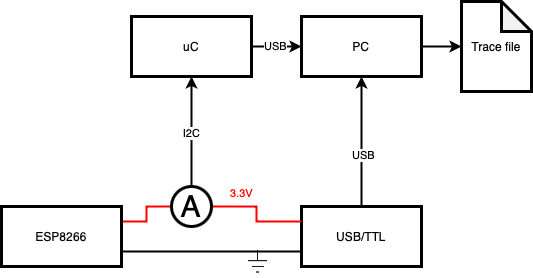
\includegraphics[width = \linewidth]{fig/experimental_setup.png}
    \caption{Setup to measure the current consumption of the ESP8266.}
    \label{fig:experiment_setup}
\end{figure}

The Amperemeter consisted of an INA219 module together with a shunt resistor of $R_{shunt} = 2.2 \Omega$.
With a maximum current consumtion of $I_{max}=170 mA$ \cite{espressif_inc_esp8266_2016}, the maximum voltage drop $U_{shunt_{max}}$ on $R_{shunt}$ is $374mV$.
\begin{align*}
    U_{shunt_{max}} &= I_{max} * R_{shunt}\\
    U_{shunt_{max}} &= 170mA * 2.2 \Omega\\
    U_{shunt_{max}} &= 374mV
\end{align*}

This still leaves $3.3V - 0.374V = 2.926V$ for the ESP8266-01 which is slightly below the specified voltage range of $3V$ to $3.3V$ \cite{espressif_inc_esp8266_2016}.
However, we had no issues like brownouts during the experiments that were caused by this lack of voltage.\\
The INA219 measured the current consumption with a frequency of $f_{INA} = 500Hz$.
A higher sampling rate would result into more accurate results but to prove the
described power saving concepts it is accurate enough.
In addition, we added a direct connection between the ESP8266-01 and the measurement setup to optionally log the relevant parts.



\subsection{Sleep modes}

\subsubsection{Experimental setup}
A common use case of a battery powered device is a temperature sensor.
Therefore, we used the following experimental setup:
\textit{The device should measure the temperature with an interval of $T_{measure} = 15min$.
MQTT should be used to publish the measured data to other devices.}

Fig. \ref{fig:experiment_modem_light_sleep} shows the test programm for the modem and light sleep.
The step \textit{setRandomMacAddress} makes sure that the ESP8266-01 always gets a new IP address.

\begin{figure}[H]
    \centering
    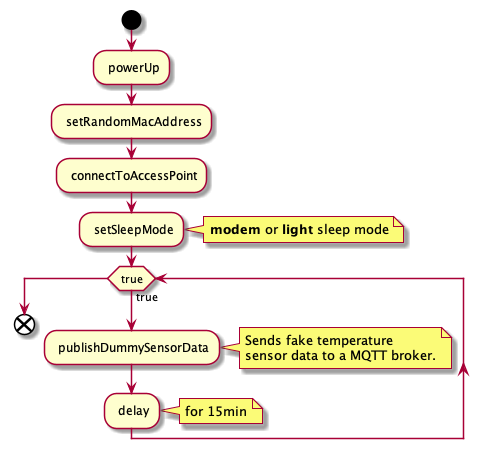
\includegraphics[width = 0.7 \linewidth]{fig/sequence_modem_light_sleep.png}
    \caption{Experimental setup for modem and light sleep.}
    \label{fig:experiment_modem_light_sleep}
\end{figure}

Fig. \ref{fig:experiment_deep_sleep} describes the experimental setup that we used to perform the tests with the deep sleep mode.
After the \textit{enterDeepSleep} step, the ESP8266-01 sleeps for $15min$ and restarts the sequence again.
The difference between deep sleep and modem / light sleep mode is, that the controller restarts the programm everytime it wakes up.\\
TODO: CITE\\
\begin{figure}[H]
    \centering
    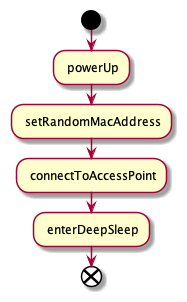
\includegraphics[width = 0.7 \linewidth]{fig/sequence_deep_sleep.png}
    \caption{Experimental setup for deep sleep.}
    \label{fig:experiment_deep_sleep}
\end{figure}

\subsubsection{Modem sleep}
As mentioned in \ref{sec:modem_sleep}, the ESP8266-01 automatically disables the modem when there is no data transmission required.
During transmission the module takes around $80mA$. During modem sleep, $20mA$ are needed.
The modem wakes up every $100ms$ (beacon interval) to keep the connection to the access point established.
Fig. \ref{fig:beacon_interval} shows the beacon interval of $100ms$. 
The same behavior was observed in \cite{montori_is_2017}.

\begin{figure}[H]
    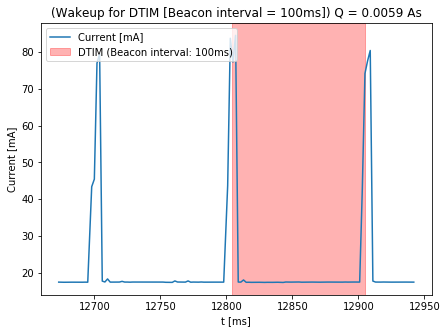
\includegraphics[width = \linewidth]{fig/beacon_interval.png}
    \caption{The power consumption increases to $\approx 80mA$, everytime a beacon arrives.}
    \label{fig:beacon_interval}
\end{figure}

\subsubsection{Light sleep}
As described in \ref{sec:light_sleep}, the light sleep mode disables the CPU when no task has to be processed.
When a task has to be processed, the ESP8266-01 switches back into modem sleep.
Fig. \ref{tab_sleep_modes} shows the change from light sleep (green) to modem sleep (red).
It is clear to see that the ESP8266-01 still needs a lot of power when a beacon arrives (every $100ms$).

\begin{figure}[H]
    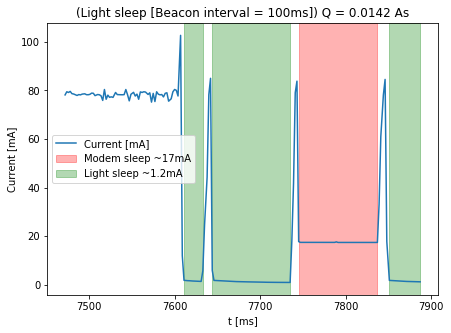
\includegraphics[width = \linewidth]{fig/light_sleep.png}
    \caption{During the light sleep mode, the power consumption of the ESP8266 is drops to 1.2mA.}
    \label{fig:light_sleep}
\end{figure}

\subsubsection{Deep sleep}
The deep sleep mode is the most efficient sleep mode, as described in \ref{sec:deep_sleep}. 
We achieved a power consumption of only $20 \mu A$. 
However, the ESP8266-01 takes a long time to reconnect to the WiFi network after waking up.
Fig. \ref{fig:deep_sleep} shows the power consumtion during the sleep and operating phase.
\begin{figure}[H]
    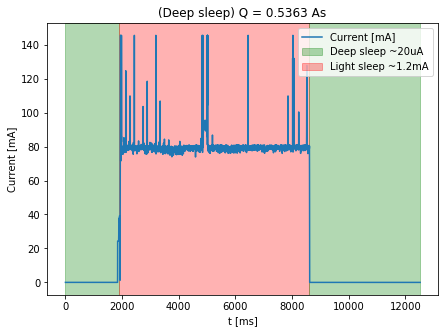
\includegraphics[width = \linewidth]{fig/deep_sleep.png}
    \caption{During deep sleep mode (green), the power consumption drops to $20 \mu A$}
    \label{fig:deep_sleep}
\end{figure}

\subsection{DHCP and static IP}
To analyse the power consumption when connecting via DHCP or with a static IP, we monitored the current of an average connection process.\\

\subsubsection{Experimental setup}
The sequence of the test program for DHCP is the same as Fig. \ref{fig:experiment_deep_sleep} shows.
Fig. \ref{fig:experiment_static_ip} shows the sequence when conducting the experiment using a static IP address.
The ESP8266-01 WiFi library provides functionality to set a static IP address.
\begin{figure}[H]
    \centering
    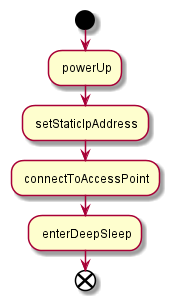
\includegraphics[width = 0.35 \linewidth]{fig/sequence_static_ip.png}
    \caption{Experimental setup for use of a static IP.}
    \label{fig:experiment_static_ip}
\end{figure}

\subsubsection{DHCP}
As shown in Fig. \ref{fig:dhcp}, the establishment of the connection to the network by using DHCP takes $\approx 5.5 s$.
In average, the average current consumption is $\approx 68.9 mA$ and in total, it consumes about $0.3545 As\ (\sigma = 0.00065$) as seen in Fig. \ref{fig:dhcp_boxplot}.
It is mentionable that in this case, everytime the device connects to the network, it gets a new IP address.
This happens because the lease time runs out before the device reconnects again.
This can be optimized by setting longer lease times.
When the lease time is long enough and the device doesn't get a new IP address, it takes around the same energy as using a static IP address.\\

\begin{figure}[H]
    \centering
    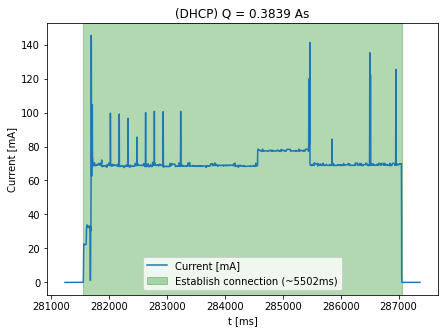
\includegraphics[width =\linewidth]{fig/dhcp.png}
    \caption{The establishment of the connection with DHCP takes $\approx 5.5s$.}
    \label{fig:dhcp}
\end{figure}

\subsubsection{Static IP address}
In Fig. \ref{fig:static_ip} a connection cycle to the WiFi network by using a static IP address is shown.
The connection to the WiFi network by using a static IP address takes $\approx 4 s$.
The average current consumption is $\approx 68.9 mA$.
As the establishment of the connection takes less time, it consumes about $0.2821 As\ (\sigma = 0.00085)$  in total, as seen in Fig. \ref{fig:dhcp_boxplot}.
The duration of the establishment of the connection is shorter, because there is no commnucation with the DHCP server needed.

\begin{figure}[H]
    \centering
    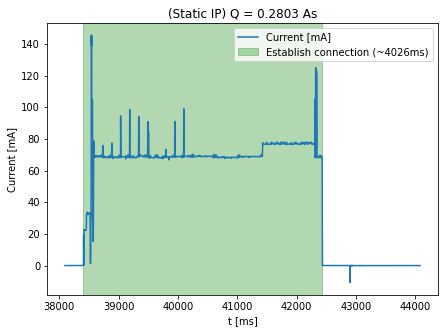
\includegraphics[width =\linewidth]{fig/static_ip.png}
    \caption{The establishment of the connection with a static IP takes $\approx 4s$.}
    \label{fig:static_ip}
\end{figure}

\begin{figure}[H]
    \centering
    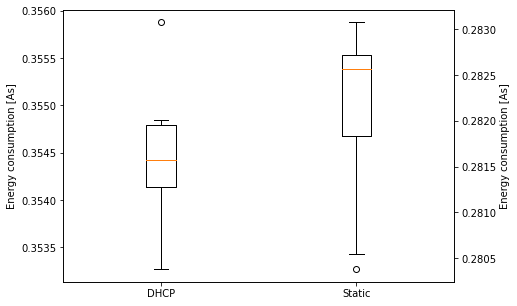
\includegraphics[width =\linewidth]{fig/dhcp_static_boxplot.png}
    \caption{$As$ of one connection interval DHCP (left) and static IP (right).}
    \label{fig:dhcp_boxplot}
\end{figure}


\subsection{UDP / TCP}
To analyse the power consumption while sending data to an client we prepared a 
experiment where we send data in a loop to a client over TCP and UDP.\\

\subsubsection{Experimental setup}
To measure the power consumption we had to extend the setup from Fig.\ref{fig:experiment_setup}.
Because the ESP8266 verified its connection to the access point while idle.
To distinguish between the verifying of the connection and the transmitting of
data we log the transmitting process.
In order to obtain only the meaningful parts of the measurements,
we have prepared a trigger via the I/O pins. While the ESP is transmitting,
the PIN 2 goes high.
On the other side the microcontroller logs the lines with 1 when the pin 1 gets current.
\newline
\begin{figure}[h]
\centering
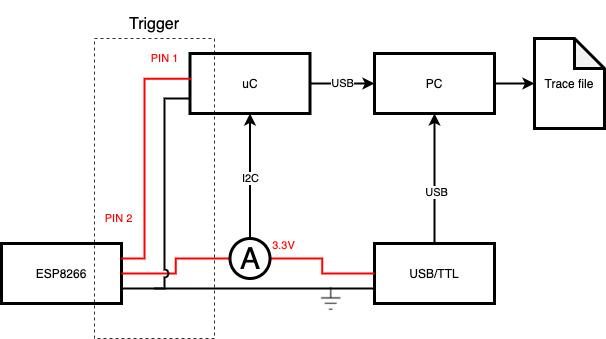
\includegraphics[width = 0.90 \linewidth]{fig/udp_tcp/experimental_setup_udp_tcp.png}
\caption{Setup to measure the current consumption while sending data with the ESP8266.}
\label{fig:experiment_udp_tcp}
\end{figure}
\subsubsection{TCP}
In order to analyze the power consumption when sending data via UDP,
we have prepared a function that transfers data from an ESP8266 to a PC via a WiFi connection.
Whithen we listens to an open port with netcat.
To study the power consumption of TCP,
we will send data to a client over TCP using the ESP8266WiFi library.
In our experiment we prepared random packets to disable the TCP chaching system.
We then processed 100 iterations of the function in Fig.\ref{fig:tcp_uml}
to geather enough values.
\begin{figure}[h]
\centering
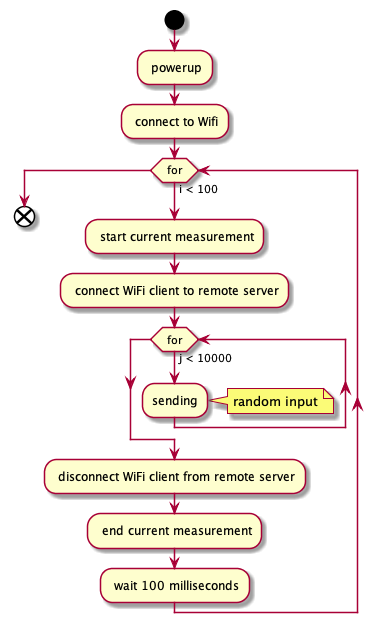
\includegraphics[width = 0.7 \linewidth]{fig/udp_tcp/tcp_uml.png}
\caption{process to sending data over TCP}
\label{fig:tcp_uml}
\end{figure}
\newline\newline
As expected, when we send data over TCP, we get a lot of different results.
This is because we have to wait for the recipient response to send the data.
\linebreak\linebreak
\begin{table}[htbp]
\begin{center}
\caption{Results TCP}
\label{tab:table1}
\renewcommand{\arraystretch}{1.8}
\begin{tabular}{l|c|r}
& \textbf{time [ms]} & \textbf{As}\\
\hline
count & 100 & 100\\
mean & 241.570 & 0.021031\\
std & 32.115403 & 0.002591\\
min & 193 & 0.016300\\
25\%  & 219 & 0.019175\\
50\% & 236 & 0.020600\\
75\%  & 257 & 0.022325\\
max & 396 & 0.032600\\
\end{tabular}
\end{center}
\end{table}
\linebreak
If we look at the results, we see that the current fluctuates a lot,
this is because TCP-buil-in system is monitoring the trasmitting 
and waiting for the recipient to receive the packet.\linebreak\linebreak
\begin{figure}[h!]
\centering
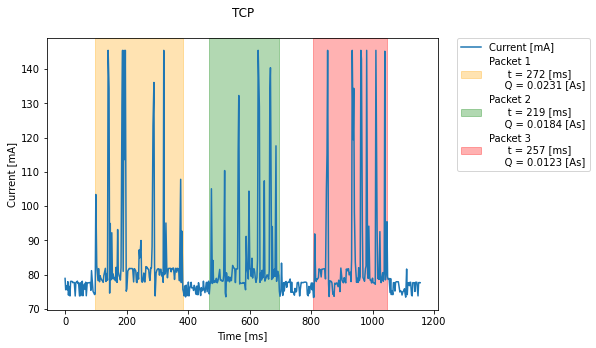
\includegraphics[width = 1 \linewidth]{fig/udp_tcp/tcp_s_m.png}
\caption{sending data over TCP}
\label{fig:tcp_s_m}
\end{figure}
\linebreak\linebreak
According these, also the elapsed time is 236$\pm$13.63\% ms
\linebreak
\begin{figure}[h!]
\centering
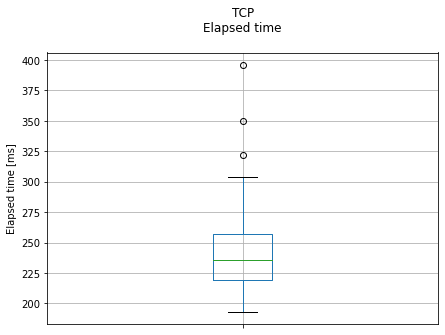
\includegraphics[width = 0.7 \linewidth]{fig/udp_tcp/tcp_boxplot_time.png}
\caption{elapsed time while sending over TCP}
\label{fig:tcp_boxplot_time}
\end{figure}
\linebreak
In addition, the power consumption is 0.0206$\pm$12.58\% As
\linebreak
\begin{figure}[h!]
\centering
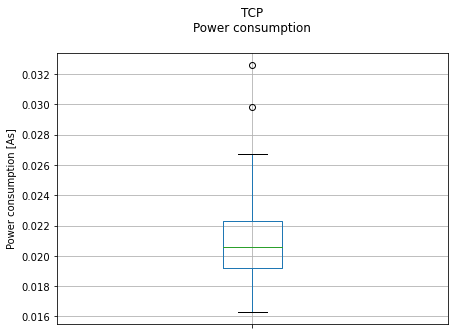
\includegraphics[width = 0.7 \linewidth]{fig/udp_tcp/tcp_boxplot_As.png}
\caption{ampere seconds while sending over TCP}
\label{fig:tcp_boxplot_As}
\end{figure}
\pagebreak
\subsubsection{UDP}
To analyse the power consumption while sending data over UDP we prepared a procedure which
transfer data from an ESP8266 to a generic notbook  via UDP from the WiFiUdp library.
In order to be able to compare with TCP, we create the process in Fig.\ref{fig:udp_uml}
\begin{figure}[h]
\centering
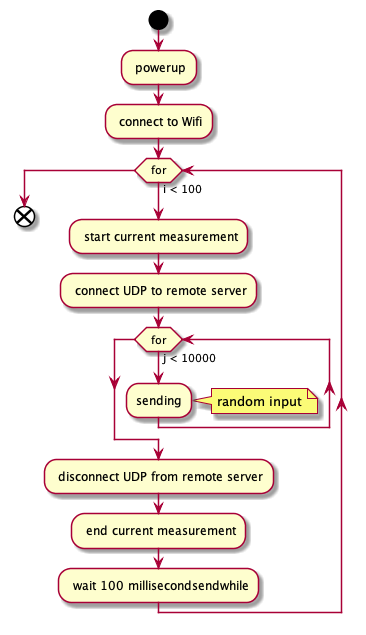
\includegraphics[width = 0.7 \linewidth]{fig/udp_tcp/udp_uml.png}
\caption{process to sending data over UDP}
\label{fig:udp_uml}
\end{figure}
\newline\newline
As expected, when we send data over UDP, we get more uniform values.
\linebreak\linebreak
\begin{table}[htbp]
\begin{center}
\caption{Results UDP}
\label{tab:table1}
\renewcommand{\arraystretch}{1.8}
\begin{tabular}{l|c|r}
& \textbf{time [ms]} & \textbf{As}\\
\hline
count & 100 & 100\\
mean & 95.970 & 0.009227\\
std & 1.058444 & 0.000581\\
min & 94 & 0.008200\\
25\% & 95 & 0.008800\\
50\% & 96 & 0.009100\\
75\% & 97 & 0.009600\\
max & 98 & 0.010900\\
\end{tabular}
\end{center}
\end{table}
\linebreak
If we look at the results, we see that the current is almost stable,
this is because UDP is not waiting for the recipient to receive the packet.
When it starts it sends the Packages simultaneously.\linebreak\linebreak
\begin{figure}[h!]
\centering
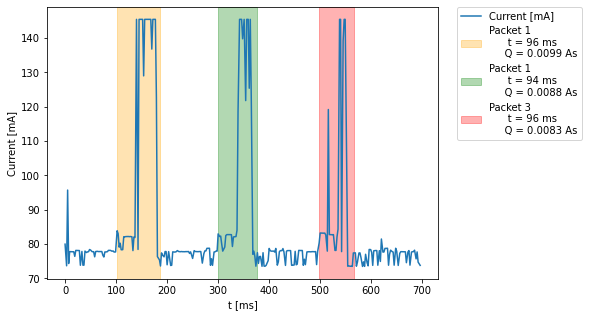
\includegraphics[width = 1 \linewidth]{fig/udp_tcp/udp_s_m.png}
\caption{sending data over UDP}
\label{fig:udp_s_m}
\end{figure}
\linebreak\linebreak
According these, also the elapsed time is 96$\pm$1.10\% ms
\linebreak
\begin{figure}[h!]
\centering
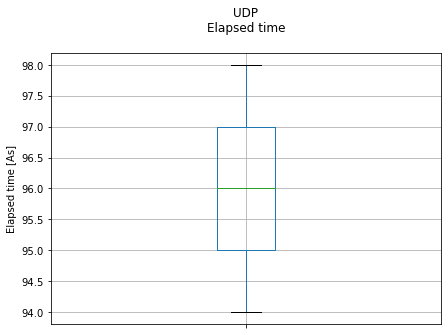
\includegraphics[width = 0.7 \linewidth]{fig/udp_tcp/udp_boxplot_time.png}
\caption{elapsed time while sending over UDP}
\label{fig:udp_boxplot_time}
\end{figure}
\linebreak
In addition, the power consumption is 0.0091$\pm$6.38\% As
\linebreak
\begin{figure}[h!]
\centering
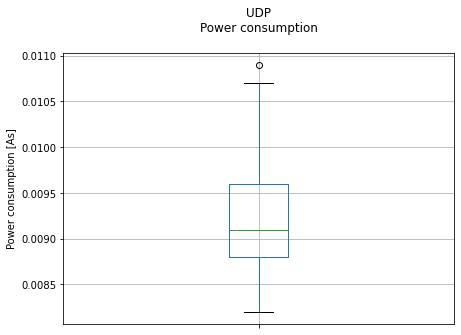
\includegraphics[width = 0.7 \linewidth]{fig/udp_tcp/udp_boxplot_As.png}
\caption{ampere seconds while sending over UDP}
\label{fig:udp_boxplot_As}
\end{figure}
\pagebreak

\section{Results}


\subsection{DHCP and static IP}
When choosing between using DHCP or a static IP, the use of a static IP is definitely less power consuming. 
As seen in Fig. \ref{fig:dhcp} the connection time using DHCP is about 1.5 seconds longer compared to the connection time of using a static IP address as shown in Fig. \ref{fig:static_ip}.
Although, it is a huge factor how long the DHCP leases are.\\
A little example: You have an ESP8266-01 that is in deep sleep and wakes up every half an hour. You are using DHCP to get an IP address. 
The DHCP lease is about 20 minutes, so everytime the device wakes up and connects to the internet, a new IP address is given by the DHCP server and therefore more energy is consumed.
Is the DHCP lease about one day, a new IP address is given only once per day and on the other remaining connection establishments, the same IP address is given, so it's consuming roughly the same energy as when using a static IP address.
As seen in Fig. \ref{fig:static_boxplot}, using a static IP address consumes about 0.078$mAh$ everytime a new connection is established.
In comparison, the use of DHCP is consuming about 0.098$mAh$ in total as seen in Fig. \ref{fig:dhcp_boxplot}.
In summary. using a static IP address instead of DHCP consumes about 20.5\% less energy and when thinking of a device that wakes up 48 times a day, this will make a huge impact on the battery life.

\subsection{UDP / TCP}
To analyze the difference in power consumption between the two transmission methods,
we compare them. In the analysis we pay attention to the elapsed time and the power consumption while the
ESP8266 transmits. In the first comparsion, we compare 100 trasmitting cicles.
\linebreak
\begin{table}[H]
    \begin{center}
    \caption{Comparison TCP UDP}
    \label{tab:table3}
    \renewcommand{\arraystretch}{1.8}
    \begin{tabular}{l|c|c|r}
    & \textbf{TCP} & \textbf{UDP} & \textbf{difference} \\
    & \multicolumn{2}{c|}{elapsed time [ms]} & \textbf{\%}\\
    \hline
    count & 100 & 100 & \\
    mean  & 241.57 & 95.97 & 39.73 \\
    std   & 32.115403 & 1.058444 & 3.30 \\
    min   & 193.0 & 94.0 & 48.70 \\
    25\%  & 219.0 & 95.0 & 43.38 \\
    50\%  & 236.0 & 96.0 & 40.68 \\
    75\%  & 257.0 & 97.0 & 37.74 \\
    max   & 396.0 & 98.0 & 24.75 \\
    \end{tabular}
    \end{center}
\end{table}
\begin{figure}[H]
    \centering
    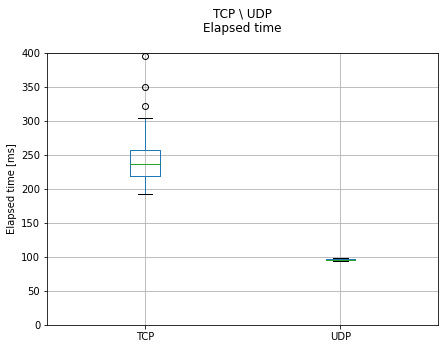
\includegraphics[width = 0.9 \linewidth]{fig/udp_tcp/udp_tcp_boxplot_time.png}
    \caption{Elapsed time when sending data over TCP and UDP}
    \label{fig:udp_tcp_boxplot_time}
    \end{figure}
If we compare the elapsed time spent sending the 1000 bytes,
we can save 96.0048$\pm$11.145 ms for a send cycle.
As shown in Table\ref{tab:table3},
we see that the range between the maximum and minimum send time for UDP is also much smaller.
As described in Chapter \ref{udp:sci}, UDP has less overhead when sending.
That's why it doesn't need energy to monitor sending cycle.
\begin{table}[H]
    \begin{center}
    \caption{Comparison TCP UDP}
    \label{tab:table4}
    \renewcommand{\arraystretch}{1.8}
    \begin{tabular}{l|c|c|r}
    & \textbf{TCP} & \textbf{{UDP}} & \textbf{difference} \\
    & \multicolumn{2}{c|}{ power consumption [As]} & \textbf{\%}\\
    \hline
    count & 100 & 100 & \\
    mean   & 0.021031 & 0.009227 & 43.87 \\
    std    & 0.002591 & 0.000581 & 22.42 \\
    min    & 0.0163 & 0.0082 & 50.31 \\
    25\%   & 0.019175 & 0.0088 & 45.89 \\
    50\%   & 0.0206 & 0.0091 & 44.17 \\
    75\%   & 0.022325 & 0.0096 & 43.00 \\
    max    & 0.0326 & 0.0109 & 33.44 \\
    \end{tabular}
    \end{center}
\end{table}
\begin{figure}[H]
    \centering
    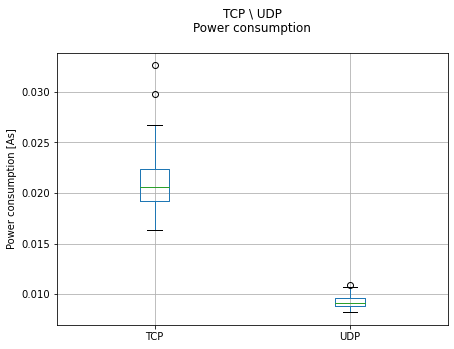
\includegraphics[width = 0.9 \linewidth]{fig/udp_tcp/udp_tcp_boxplot_As.png}
    \caption{Power connsumption when sending data over TCP and UDP}
    \label{fig:udp_tcp_boxplot_As}
    \end{figure}
In Table\ref{tab:table4} we compared the elapsed time while the ESP8266 sends.
As expected, we get the same result.
UDP requires only 44.03\%$\pm$6.07\% of the time compared to TCP.
This gives us a saving of 0.00907018$\pm$0.00125 As while sending 1000 bytes.
For example, in Fig.\ref{fig:udp_tcp_s_m},
we compare the iteration 50 to see the differences between the two.
The power consumption of UDP increases the first time the connection
is started and the second part is exactly when it sends.
In contrast, TCP requires much more power to establish the connection and waits before sending.
\begin{figure}[H]
    \centering
    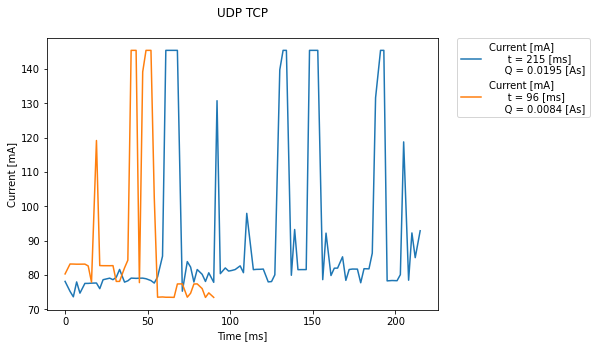
\includegraphics[width = 1 \linewidth]{fig/udp_tcp/udp_tcp_s_m.png}
    \caption{Sending data over TCP and UDP}
    \label{fig:udp_tcp_s_m}
    \end{figure}



\section{Conclusions}

\subsection{Figures and Tables}

\section*{Acknowledgment}

The preferred spelling of the word ``acknowledgment'' in America is without 
an ``e'' after the ``g''. Avoid the stilted expression ``one of us (R. B. 
G.) thanks $\ldots$''. Instead, try ``R. B. G. thanks$\ldots$''. Put sponsor 
acknowledgments in the unnumbered footnote on the first page.


\printbibliography
\end{document}
